\documentclass[../report.tex]{subfiles}
\begin{document}
\section{Building and Running the Application}
\subsection{Building}

	This step is not strictly necessary to run the application as it is available as pre-built docker images but is included for completeness.  To build (probably) requires a Unix like environment (e.g. Linux or Mac OS), Python 3.5+ with pip, GNU make and docker.
	
\begin{verbatim}
	$ cd seismic-detector
	$ python3 -m virtualenv .
	$ source bin/activate
	$ pip install numpy
	$ make clean sdist docker
\end{verbatim}

\subsection{Running}

\subsubsection{Starting \& Stopping} \label{sec:start-stop}

	To run the application pre-built requires docker and docker-compose.  It is hosted on the Docker Hub so it does not need to be built first.
	
	From the root of the project (on writeable media such as a hard disk), invoke \texttt{docker-compose up -d}.
	
\begin{verbatim}
	$ docker-compose up -d
	docker-compose up -d
	Creating network "seismic_default" with the default driver
	Creating seismic_api_1
	Creating seismic_minio_1
	Creating seismic_postgres_1
	Creating seismic_redis_1
	Creating seismic_worker_1
	Creating seismic_interface_1
\end{verbatim}

	The application should now be available via a browser on \texttt{http://localhost:8080}.  To terminate, call \texttt{docker-compose down}.

\newpage	
\subsubsection{Using the Application} \label{sec:using-application}
	
\begin{figure}[H]
	\centering
	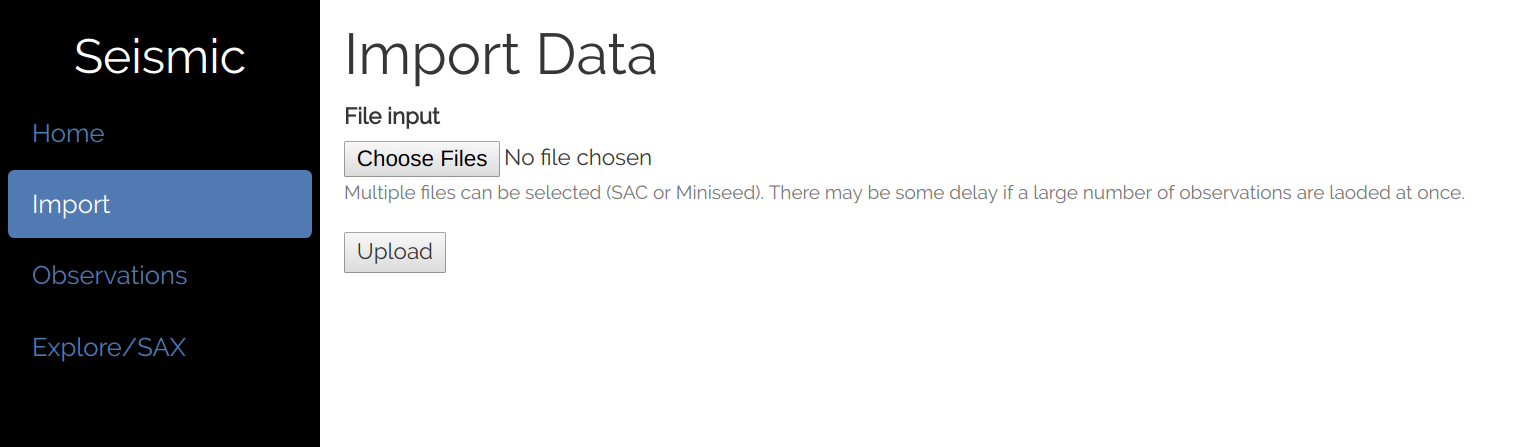
\includegraphics[width=1\linewidth]{img/run-import}
	\caption{Importing Observations}
\end{figure}

	From the homepage, select \textbf{Import} from the menu.  Then click on \textbf{Choose Files} and select some observations (there are some under \texttt{/sample/\_all} in the included source).  Then hit \textbf{Upload}, if all was successful, you will see a list of the files uploaded in green.

\begin{figure}[H]
	\centering
	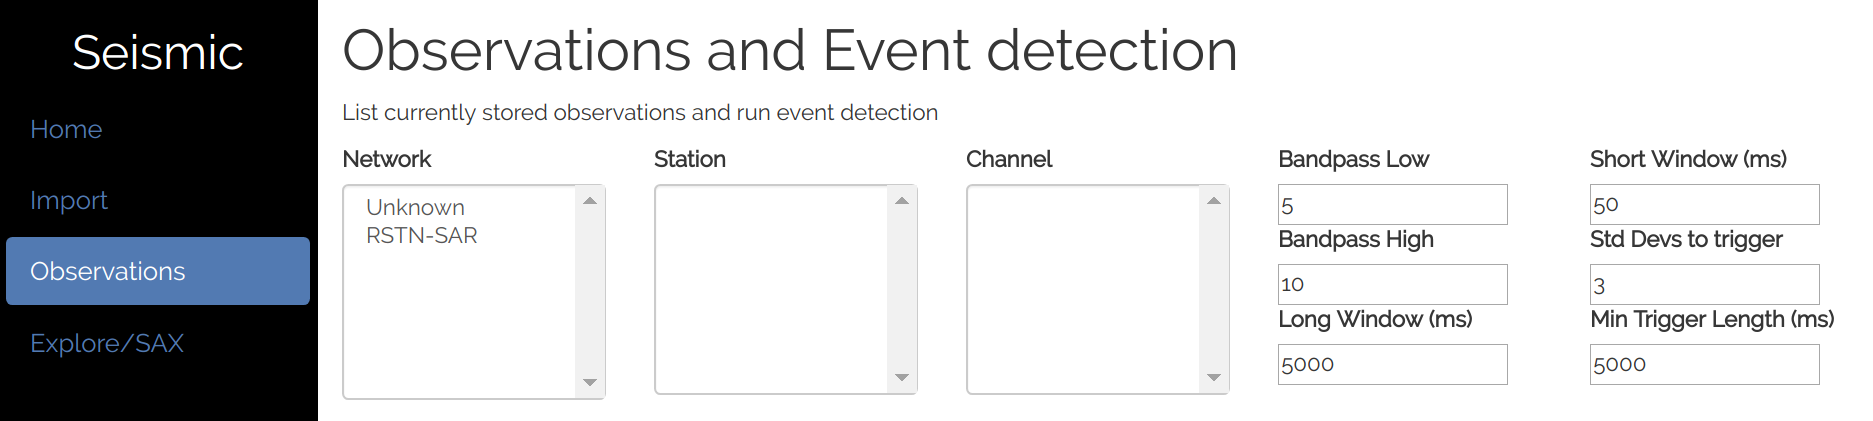
\includegraphics[width=1\linewidth]{img/run-observations}
	\caption{Searching Observations (1)}
\end{figure}

	Once the files have been uploaded, click on \textbf{Observations}.

\begin{figure}[H]
	\centering
	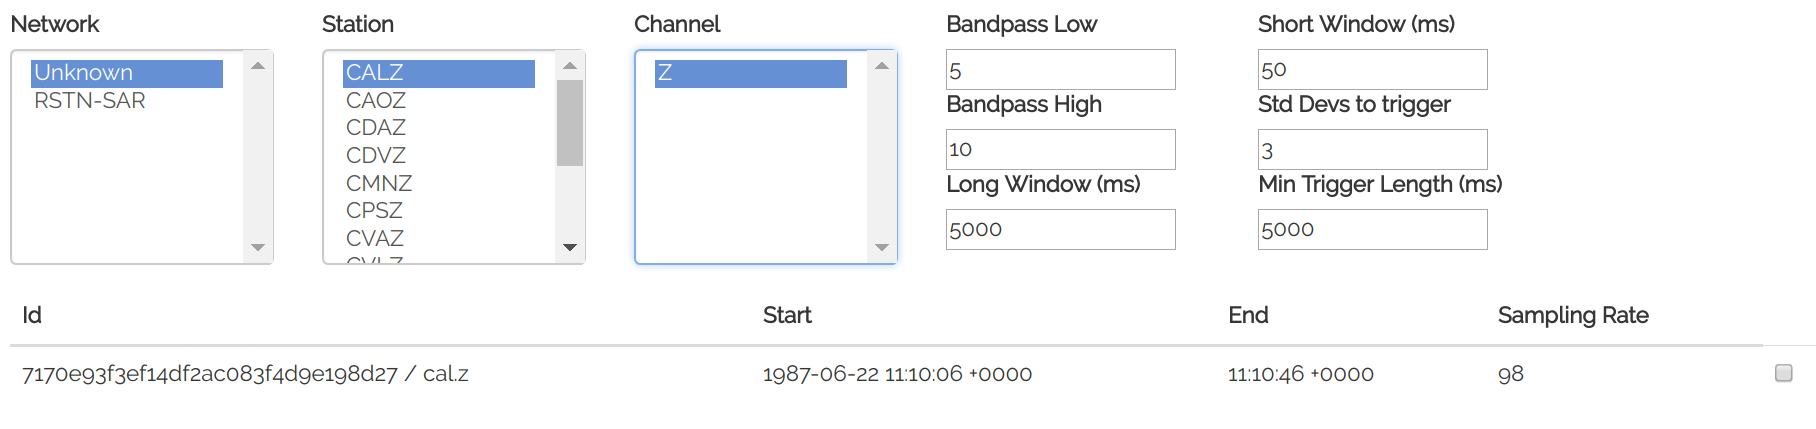
\includegraphics[width=1\linewidth]{img/run-select}
	\caption{Searching Observations (2)}
	\label{fig:run-select}
\end{figure}

	Then select a \textit{Network}, \textit{Station} and \textit{Channel} to see observations that match your criteria (\cref{fig:run-select}).

\begin{figure}[H]
	\centering
	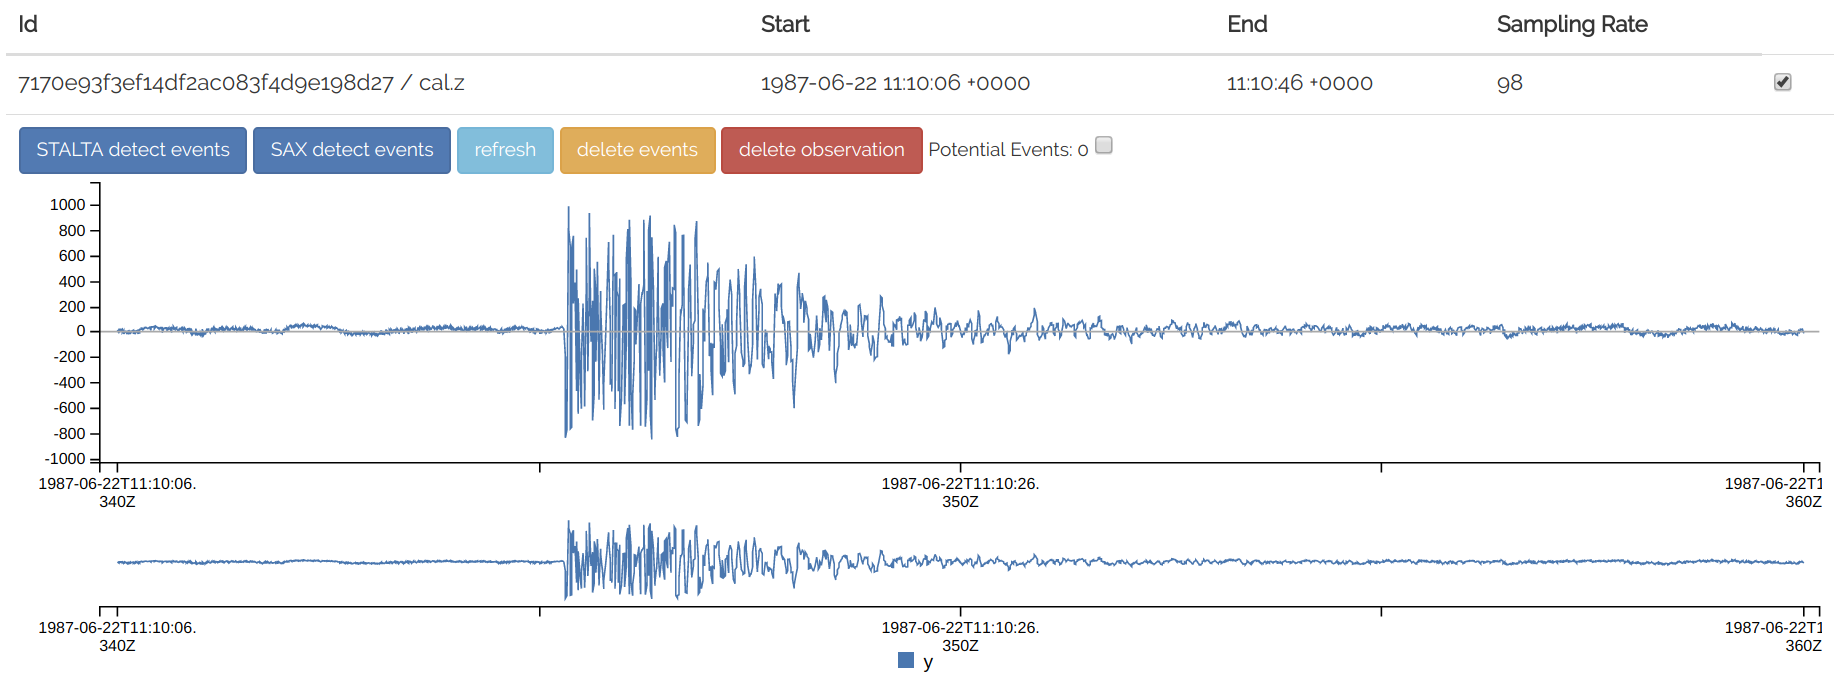
\includegraphics[width=1\linewidth]{img/run-render}
	\caption{Viewing an Observation}
	\label{fig:run-render}
\end{figure}

	By ticking the checkbox next to an event, you are presented with a rendering of the whole observation and some controls (\cref{fig:run-render}).

\begin{figure}[H]
	\centering
	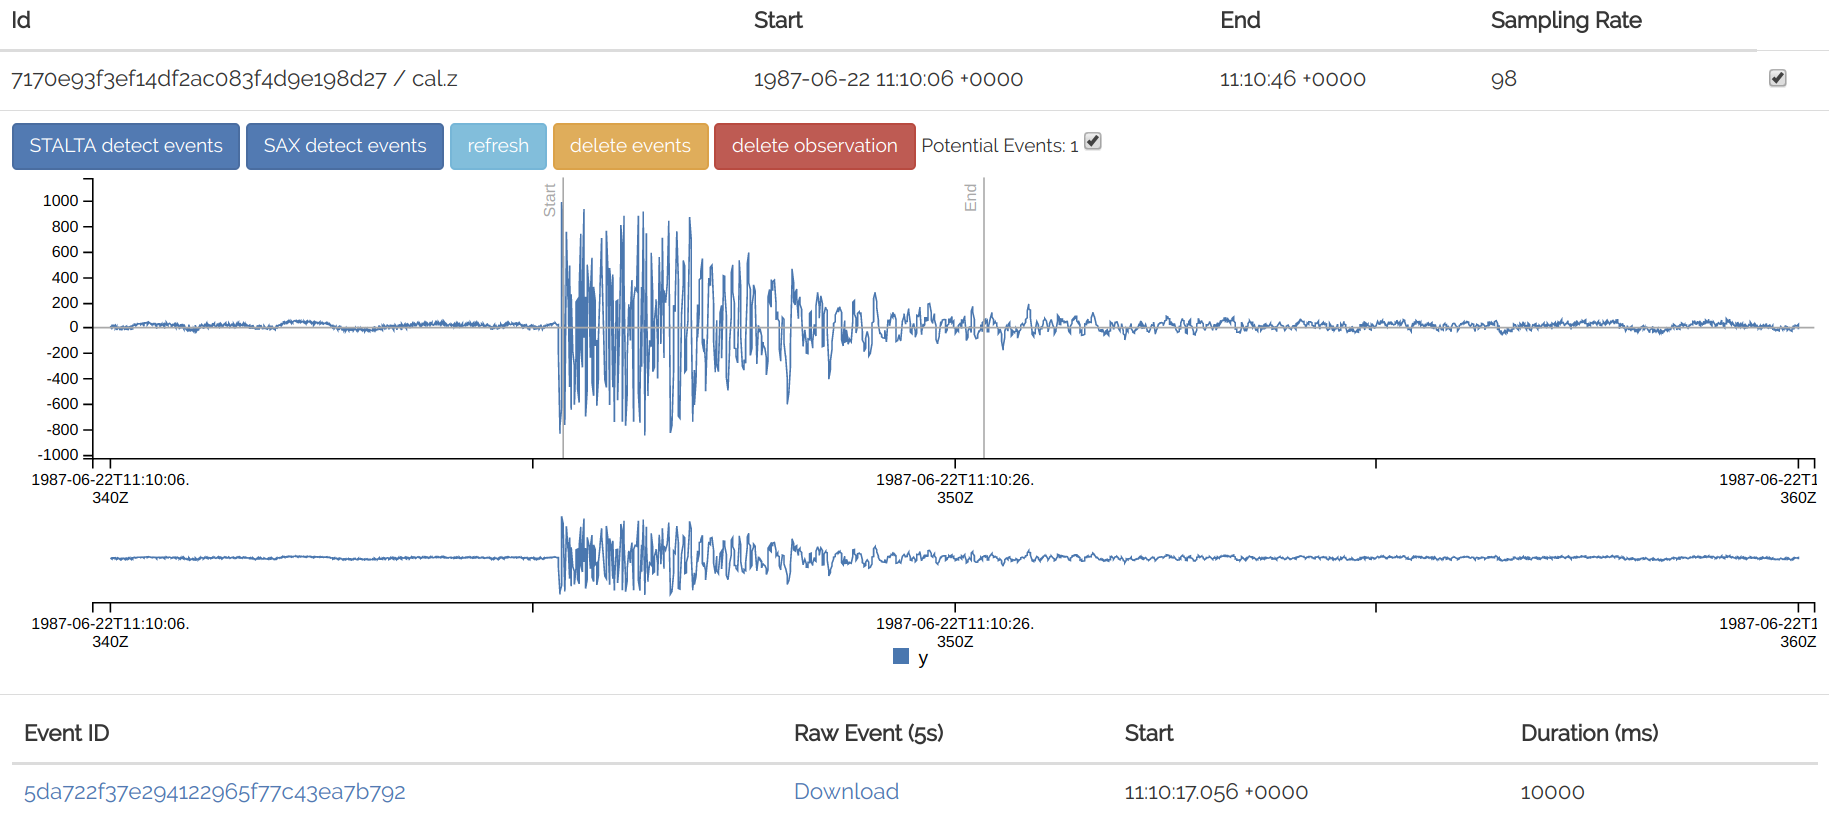
\includegraphics[width=1\linewidth]{img/run-detected}
	\caption{Detecting Events}
	\label{fig:run-detected}
\end{figure}

	To detect an event either by STA/LTA or SAX, hit the relevant control and then hit the light blue \textbf{Refresh} button next to them to see if there were any potential events found.  If there were, you can tick the box next the the number of events to see them displayed on the graph (\cref{fig:run-detected}).

\begin{figure}[H]
	\centering
	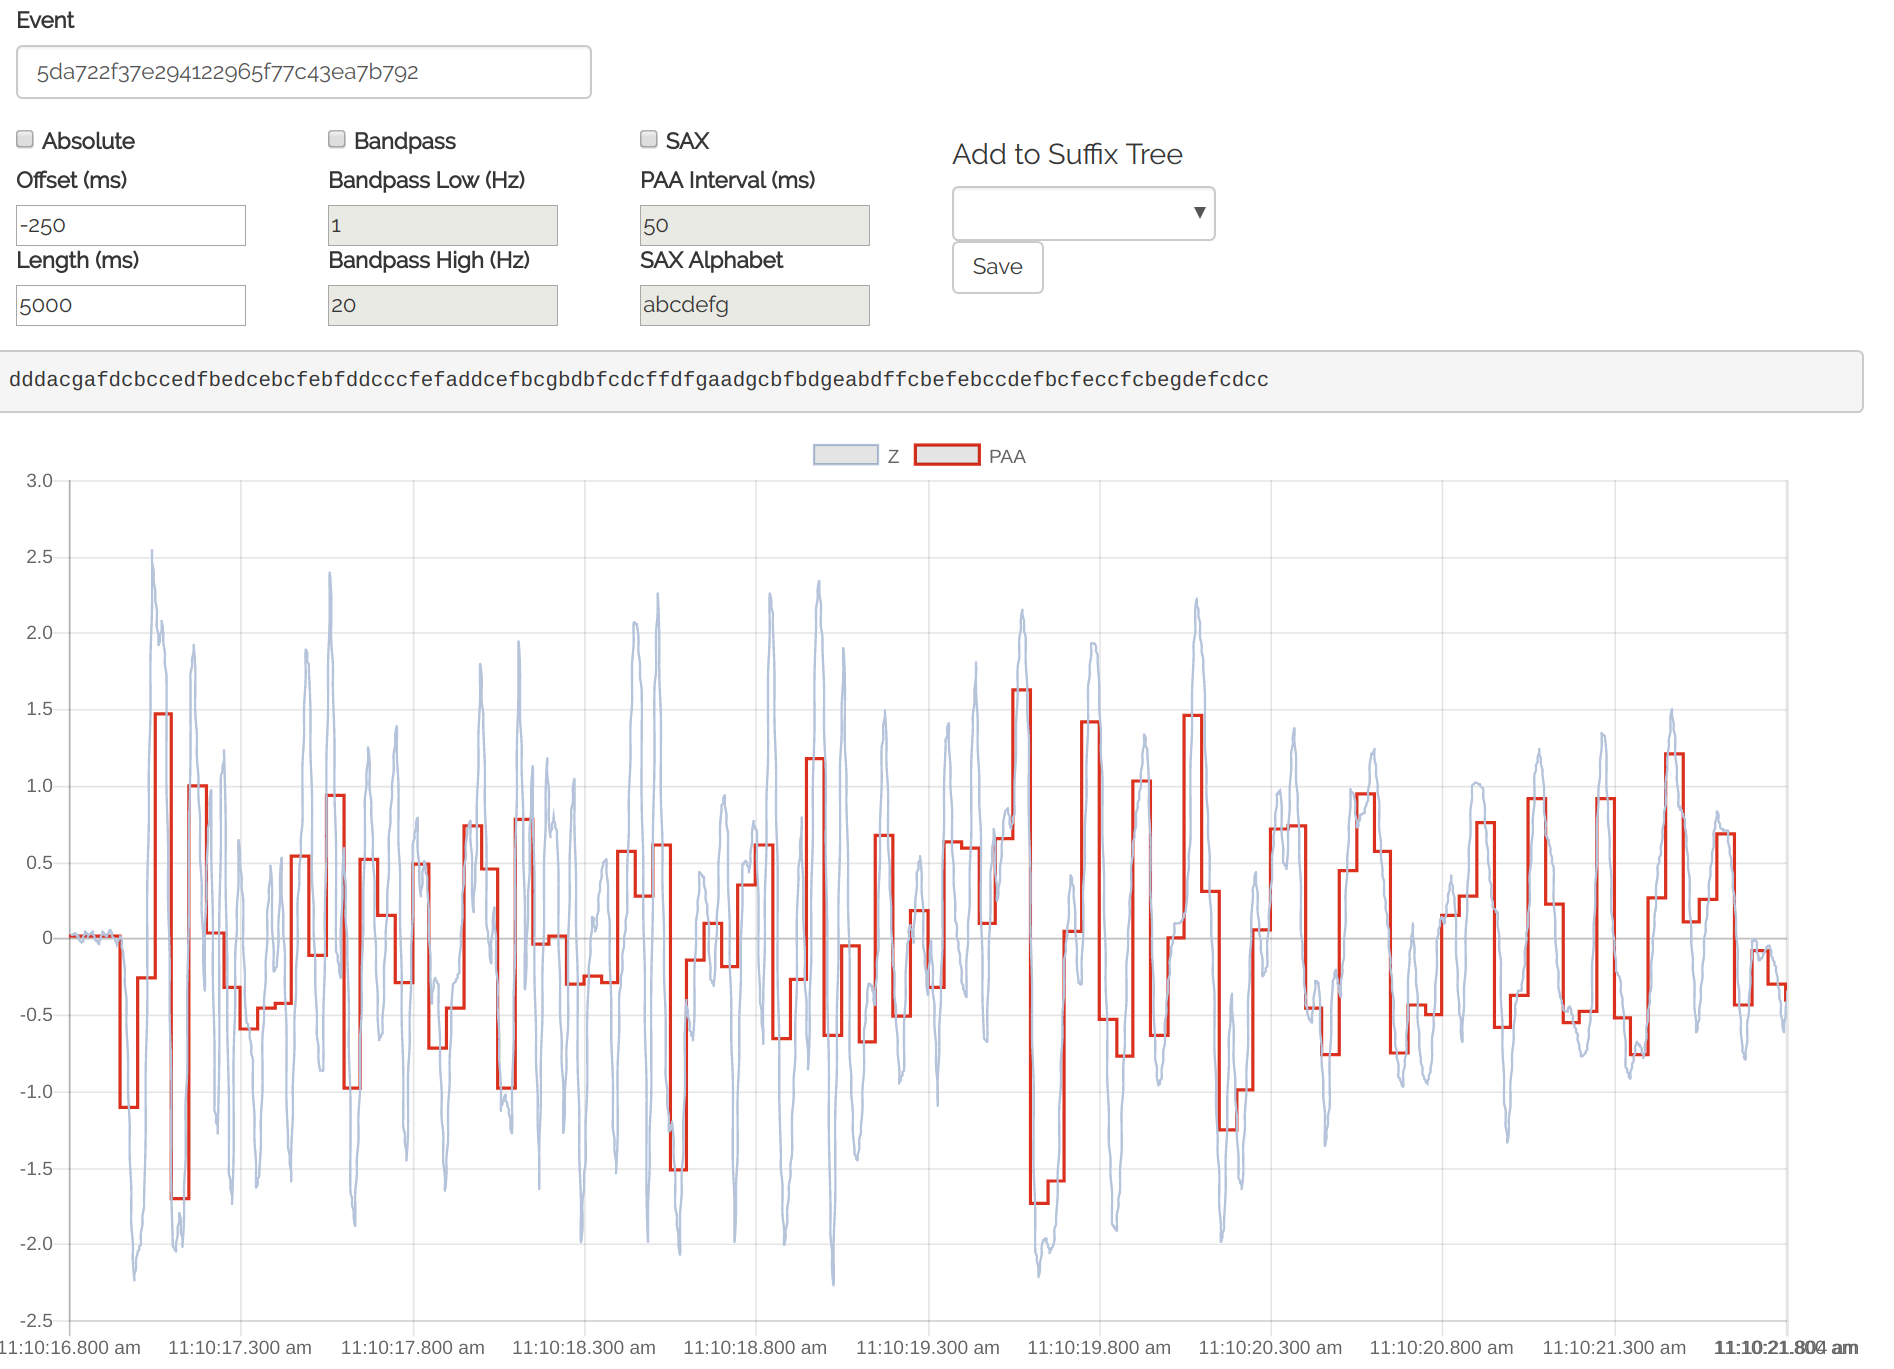
\includegraphics[width=1\linewidth]{img/run-event}
	\caption{Viewing PAA \& SAX}
	\label{fig:run-event}
\end{figure}

	To see the event in more detail and to view the PAA/SAX process, you can click on the event ID for that event (\cref{fig:run-event}).


\end{document}